\chapter{Introducción}

%\juani{IMPORTANTE, MIRA SI HAY UN FORMATO PARA EL PROYECTO. EN LA PÁGINA DE LA UAL HAY UNA PLANTILLA QUE ES LIGERAMENTE DIFERENTE A ESTA. ES ALGO QUE SE PROPUSO DESPUÉS, PERO NO SE SI ES OBLIGATORIO UTILIZARLA. COMPRUÉBALO. DE ESA PLANTILLA TAMBIÉN PUEDES VER COMO SE MUESTRAN LOS CÓDIGOS, QUE ES DIFERENTE A LA FORMA QUE TE LO HE DICHO YO. LO MISMO TE GUSTA MÁS. AQUÍ TIENES LA PÁGINA WEB DONDE PUEDES ENCONTRARLA}
%\textbf{https://es.overleaf.com/latex/templates/memoriatfg-ual/tqmxcckfypss}


\section{Justificación}
Las aplicaciones y sitios web dedicados a la predicción meteorológica en nuestro país dependen en gran medida de los datos proporcionados por satélites geoestacionarios METEOSAT, observatorios meteorológicos, radares y una amplia variedad de equipos distribuidos en toda la península, que transmiten información a la Agencia Estatal de Meteorología de España (AEMET).

A lo largo de los años, estos datos recopilados se han vuelto notablemente más precisos gracias al avance tecnológico. Este progreso no solo se ha traducido en una mayor precisión en la información reunida, sino también en una disponibilidad más rápida y accesible de estos datos \cite{intro_1}. Históricamente, los diversos centros de observación meteorológica requerían una supervisión constante y la intervención humana para su funcionamiento. Sin embargo, en la actualidad, contamos con estaciones automatizadas que son capaces de proporcionar datos de manera continua, dejando la intervención humana solo para tareas de mantenimiento correspondientes \cite{intro_2}.

Este desarrollo tecnológico en el ámbito de la meteorología es de una importancia trascendental, y su impacto en nuestra vida cotidiana es más significativo de lo que muchas personas pueden imaginar. Nuestra vida siempre ha estado condicionada de alguna forma por las fluctuaciones climáticas. Las predicciones meteorológicas han permitido a profesionales, como agricultores, ganaderos y pescadores, llevar a cabo sus tareas de manera óptima, adaptándose y planificando sus acciones en función de las condiciones atmosféricas. Incluso para aquellos de nosotros que no estamos directamente relacionados con estos sectores, el pronóstico del tiempo sigue siendo relevante; nos ayuda a tomar decisiones cotidianas, como vestirnos adecuadamente antes de salir, planificar actividades al aire libre y mucho más. Por lo tanto, la meteorología influye de manera significativa en múltiples aspectos de nuestras vidas.

Sin embargo, a pesar de los avances tecnológicos y la mejora en las predicciones meteorológicas, aún no hemos alcanzado la perfección en este campo. ¿Por qué seguimos encontrando discrepancias? ¿Por qué a menudo vemos que dos aplicaciones ofrecen información diferente para la misma ubicación?

Estos desafíos suelen estar vinculados a dos situaciones principales: en primer lugar, la ubicación de los centros de recopilación de datos no siempre coincide exactamente con la localidad en cuestión, lo que es especialmente común en áreas rurales o pueblos pequeños. En segundo lugar, dos aplicaciones pueden utilizar la misma fuente de datos, pero sus métodos y algoritmos de predicción difieren, lo que puede dar lugar a variaciones en los resultados pronosticados \cite{intro_3}. Estos factores, junto con otros desafíos inherentes a la naturaleza cambiante del clima, explican por qué las predicciones meteorológicas, aunque avanzadas, todavía pueden presentar divergencias en ciertas circunstancias.

%\juani{David, tienes que relacionar lo que has puesto arriba con tu trabajo TFG. ¿Qué es lo que vas a hacer y porqué? Yo te he puesto algunas ideas aquí que puedes desarrollar. Trata de poner referencias en el texto.}

En nuestro caso, disponemos de una estación meteorológica en una casa inteligente (\textit{smarthome}) equipada con sensores ambientales. Esta \textit{smarthome} y sus sensores serán clave en el desarrollo de este Trabajo Fin de Grado (TFG), ya que se tratará de recopilar todos los datos relevantes para mejorar el nivel de confort de los ocupantes de la \textit{smarthome}.

%\juani{En nuestro caso, disponemos de una estación meteorológica en una casa inteligente (smarthome) equipada con sensores ambientales, lo cual  representa un elemento de gran relevancia en el marco de este Trabajo de Fin de Grado (TFG). La motivación subyacente que impulsa este trabajo y su desarrollo radica en querer aprovechar al máximo los datos recopilados por esta estación meteorológica para mejorar el nivel de confort de los ocupantes de la smarthome.}

Según la normativa ISO (Norma Internacional Organización) 7730, el confort térmico se define como "la condición de la mente en la que se expresa satisfacción con el ambiente térmico". Sin embargo, con el paso de los años, se ha ido desarrollando esta definición del confort térmico, así como sus sistemas de medición y medidas a tomar. Si bien es fundamental tener en cuenta la temperatura, luminosidad o la calidad del aire, cada vez se tienen más en cuenta variables como el diseño de un hogar optimizado para el confort térmico, el ahorro de energía o los materiales utilizados para la construcción.

La conexión entre estos dos conceptos, la meteorología y el confort en una \textit{smarthome}, es fundamental. Al comprender minuciosamente las condiciones meteorológicas actuales y futuras, podemos tomar decisiones que repercuten directamente en la calidad de vida de los residentes. Esta capacidad de anticipación se traduce en una serie de acciones que buscan optimizar el entorno de la casa en función de los pronósticos meteorológicos.

%\juani{La conexión entre estos dos conceptos, la meteorología y el confort en una vivienda inteligente, es fundamental. Al comprender minuciosamente las condiciones meteorológicas actuales y futuras, podemos tomar decisiones informadas que repercuten directamente en la calidad de vida de los residentes. Esta capacidad de anticipación se traduce en una serie de acciones que buscan optimizar el entorno de la casa en función de los pronósticos meteorológicos.}

Un ejemplo claro de esta sinergia es la adaptación automática del sistema de calefacción ante la previsión de un día particularmente frío. El sistema inteligente de la \textit{smarthome}, al tener conocimiento de estas condiciones climáticas adversas, puede activar o ajustar la calefacción para mantener una temperatura interior cómoda y agradable. Si le sumamos la monitorización de la temperatura interior y exterior, podremos reaccionar en tiempo real a cambios repentinos, en este caso, si sube la temperatura exterior pese a la predicción o si bajara aún más. Del mismo modo, en días calurosos, se pueden tomar medidas preventivas, como la activación de sistemas de refrigeración o la gestión de persianas y cortinas para mantener el interior fresco.

En definitiva, esta investigación persigue utilizar la información meteorológica recopilada por la estación en la \textit{smarthome} como un recurso clave para la toma de decisiones y la implementación de acciones automatizadas que mejoren el confort y el bienestar de los ocupantes. La interconexión entre la tecnología y la meteorología en el ámbito de las viviendas inteligentes es una vía prometedora para optimizar la calidad de vida y garantizar un ambiente interior agradable y adecuado en cualquier condición climática.

\section{Objetivos}
%\juani{En los objetivos no puedes incluir ya el lenguaje de programación que vas a utilizar. He reescrito lo que tenías. Échale un vistazo por si me he colado en algo.}

El objetivo primordial de este proyecto es asegurar y mantener un nivel óptimo de confort térmico en la smarthome de la UAL. Con el fin de cumplir con esta misión, se han delineado objetivos concretos que se enmarcan en la meta general de optimizar el confort térmico en la smarthome de la UAL, haciendo uso de los datos atmosféricos recopilados y tomando medidas adecuadas para mejorar la experiencia de los ocupantes. A continuación se detallan:

\begin{itemize}
    \item \textbf{Obtención de Datos Atmosféricos y Almacenamiento:}
    \begin{itemize}
        \item Estudio de los Sensores Actuales: Evaluación de los sensores existentes para comprender su funcionamiento y precisión.
        \item Acceso a los Sensores a través de la API: Establecimiento de un acceso a los sensores a través de la API de la smarthome para la obtención de datos meteorológicos en tiempo real.
        \item Desarrollo de un Script de comunicación: Creación de un script  que se conecte automáticamente a la API de la smarthome para recopilar y registrar datos atmosféricos.
        \item Instalación y Configuración de Bases de Datos: Implementación y configuración de bases de datos apropiadas para el almacenamiento de los datos obtenidos de los sensores.
    \end{itemize}

    \item \textbf{Visualización de Datos y Cálculo del Confort:}
    \begin{itemize}
        \item Representación Gráfica de Datos: Desarrollo de una interfaz que permita la representación visual de información meteorológica a través de gráficos y otros indicadores relevantes utilizando los datos almacenados.
        \item Investigación y Aplicación de un Modelo de Confort: Investigación y aplicación de un modelo que permita calcular el nivel de confort en la smarthome en función de los datos atmosféricos recopilados.
    \end{itemize}

    \item \textbf{Control y Modificación del Confort:}
    \begin{itemize}
        \item Desarrollo de un Script de Control: Creación de un script en Python que, basado en el nivel de confort térmico actual, tome decisiones automáticas para controlar los dispositivos de la casa y mantener o modificar el grado de confort.
        \item Comunicación con el Usuario a través del Altavoz Sonos: Implementación de una funcionalidad que informe al usuario de la casa, a través del altavoz Sonos, sobre el estado actual del confort y las acciones tomadas para ajustarlo, garantizando una comunicación efectiva y comprensible.
    \end{itemize}

    \item \textbf{Redacción de la memoria y otras tareas:}
    \begin{itemize}
        \item Investigación: búsqueda de artículos bibliográficos que respalden y justifiquen los modelos utilizados, búsqueda de dudas y documentación para los lenguajes de desarrollo y software utilizados.
        \item Redacción de la memoria: en formato LaTeX a través de OverLeaf.
        \item Reuniones con los tutores: realizadas a través de Google Meet y a lo largo del desarrollo del proyecto.
    \end{itemize} 
\end{itemize}




\section{Planificación Temporal}
%\juani{David, la idea aquí es asociar a cada uno de los objetivos que tienes en el apartado anterior una tarea. A esa tarea le das un tiempo y lo muestras gráficamente. En la plantilla del TFG que te he puesto al inicio tienes una manera para hacer la planificación temporal en latex, aunque puedes hacerla como imagenes.IMPORTANTE: LAS HORAS LAS REPARTES ENTRE LAS TAREAS COMO QUIEREAS, ESO SÍ, TIENEN QUE SUMAR AL FINAL 300 HORAS  }

Los objetivos se llevarán a cabo con una planificación de aproximadamente 309 horas en total, con la siguiente distribución en el tiempo:

\begin{figure}[h]
        \centering
        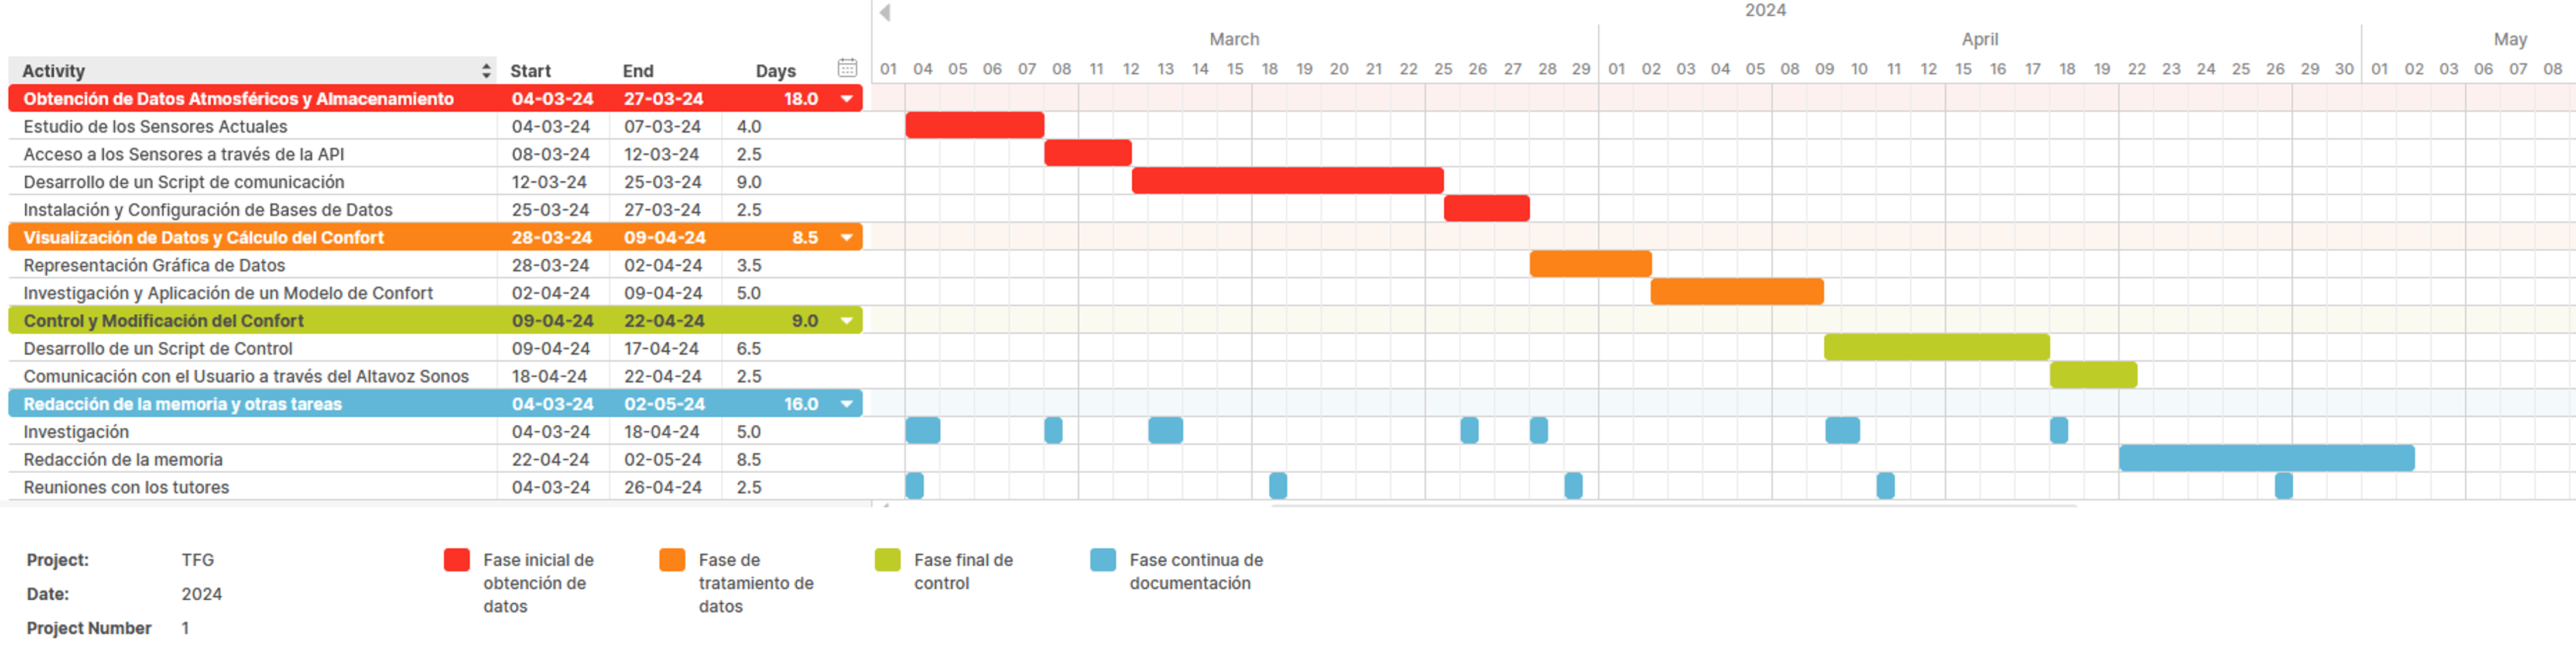
\includegraphics[width=16cm]{Imágenes/Capítulo 1/Ilustración 3. Planificación temporal.png}
        \caption{Planificación Temporal del TFG}
        \label{fig:planificacion_temporal_TFG}
    \end{figure}

\section{Estructura del documento}

El contenido del trabajo se divide en los siguientes capítulos:

\begin{itemize}
    \item \textbf{Introducción:} es la sección actual, donde se realiza una introducción y se explican los objetivos y estructura del trabajo.
    \item \textbf{Capítulo 1. Contexto del trabajo, justificación y motivación:} en este capítulo se describirán las herramientas usadas y las características de la \textit{Smarthome}.
    \item \textbf{Capítulo 2. \textit{API} y \textit{Endpoints} de la \textit{Smarthome}:} en este capítulo se tratará el acceso a los sensores de la \textit{Smarthome}, utilizando la \textit{API} de su servidor y los \textit{endpoints} que ofrece, a través de un \textit{script} en \textit{Python}.
    \item \textbf{Capítulo 3. Almacenamiento en Bases de Datos de los datos recogidos:} en este capítulo se explica cómo almacenar en las distintas bases de datos todos los datos recogidos por las sensores, a través del \textit{script} evolucionado.
    \item \textbf{Capítulo 4. Visualización de los datos en \textit{Grafana}:} en este capítulo se mostrará la interfaz de \textit{Grafana} diseñada, junto a los gráficos con los datos recatados de las bases de datos, para la revisión de la \textit{Smarthome}.
    \item \textbf{Capítulo 5. Cálculo y monitorización del Confort de la \textit{Smarthome}:} en este capítulo se estudiarán los distintos métodos de cálculo de confort y se propondrá el método elegido para este trabajo.
    \item \textbf{Capítulo 6. Control y modificación del Confort:} en este capítulo se desarrollarán los criterios elegidos para actuar sobre diferentes elementos de la \textit{Smarthome} y conseguir alcanzar un Confort óptimo, a través de la siguiente evolución del \textit{script}.
    \item \textbf{Conclusiones y mejoras:} en esta sección se plantearán tanto las conclusiones del trabajo realizado como aquellos aspectos en los que mejorar y continuar el trabajo.
\end{itemize}